\section{Divisori di frequenza}
\subsection{Montaggio e verifica}
Si è innanzitutto realizzato il circuito in \fig{div} utilizzando l'integrato SN74LS93 (un ripple counter costituito da quattro JK flip-flop), mettendo uno degli ingressi di reset ($R_{0,1}$) a terra, per poi verificarne visivamente il corretto funzionamento inviando un clock lento ($\sim \SI{1}{\Hz}$) ed osservando i LED (e dunque gli output dei flip-flop) ``contare'' ciclicamente da 0 a 15.

\begin{figure}[h]
	\centering
	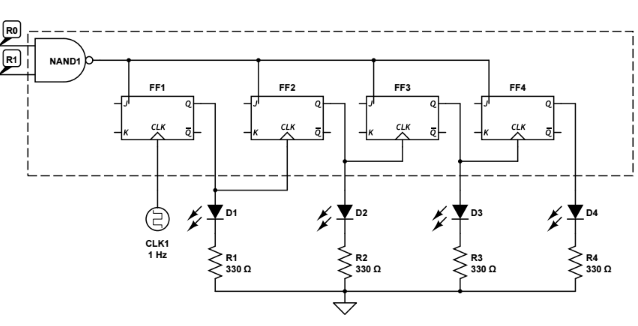
\includegraphics[scale=0.8]{divisori.png}
	\caption{Circuito divisore}
	\label{fig:div}
\end{figure}

\subsection{Verifica funzionamento divisore e misura dei tempi di ritardo.}
Effettuata la verifica precedente si è posta $f_{clock} = \SI{49.998(1)}{ \kilo \hertz}$\footnote{Questa e tutte le seguenti misure di frequenza sono state eseguite con il frequenzimetro dell'oscilloscopio per via della sua grande precisione; si è preso fino all'ultima cifra stabile con il corrispondente errore.} per procedere dunque alla misura della frequenza dei segnali in uscita ai flip-flop del contatore, ottenendo i valori in \tab{divlag}.

I segnali sono riportati in \fig{divout}. Si ha dunque come atteso un funzionamento da divisore di frequenza (con ottima precisione).

\begin{figure}[h]
	\centering
	\begin{minipage}{0.47\textwidth}
		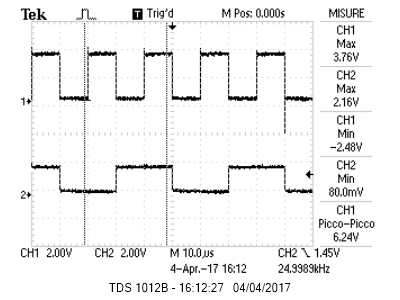
\includegraphics[scale=0.8]{divisore_2x.png}
		\\
		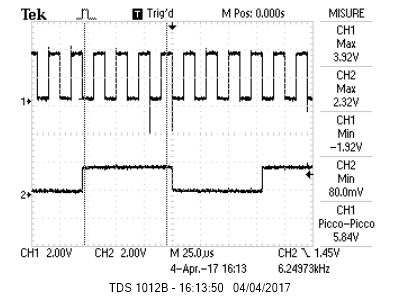
\includegraphics[scale=0.8]{divisore_8x.png}
	\end{minipage}
	\begin{minipage}{0.47\textwidth}
		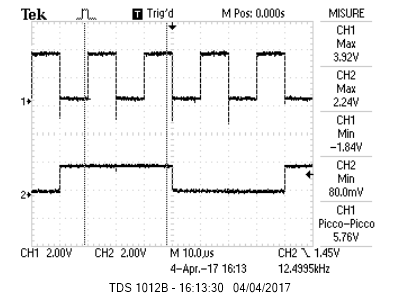
\includegraphics[scale=0.8]{divisore_4x.png}
		\\
		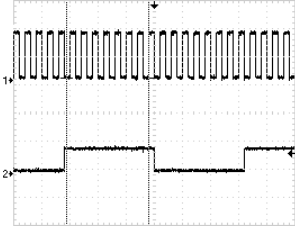
\includegraphics[scale=0.8]{divisore_16x.png}
	\end{minipage}
	\caption{Output dei quattro flip-flop del divisore (CH2) e segnale di clock (CH1).}
	\label{fig:divout}
\end{figure}

Si sono successivamente misurati\footnote{La misura è stata eseguita mediante i cursori dell'oscilloscopio.} i tempi di ritardo degli output dei flip-flop, ovvero l'intervallo temporale tra il fronte (di discesa) del clock in cui ci si attende una variazione dell'output e il fronte della variazione stessa, misurato tra i punti di tensione intermedia tra il livello alto e quello basso. I valori ottenuti sono riportati in \tab{divlag}. %qualquadra non cosa, non riesco a fargli fare la formattazione SI

\begin{table}[h]
	\centering
	\begin{tabular}{l S[table-figures-decimal=4, table-figures-uncertainty=1] S[table-figures-decimal=1, table-figures-integer=3, table-figures-uncertainty=1] S[table-figures-decimal=1, table-figures-uncertainty=1] }
		\toprule
			& {$f$ [\si{\kHz}]} & {$\Delta t_{salita}$ [\si{\ns}]} & {$\Delta t_{discesa}$ [\si{\ns}]} \\
		\midrule
		$Q_1$ & 24.999(1) & 76.0(4) & 24.2(1) \\
		$Q_2$ & 12.499(1) & 101 (1) & 30.8(2) \\
		$Q_3$ & 6.2497(1) & 110 (1) & 42.0(2) \\
		$Q_4$ & 3.1251(1) & 155 (1) & 53.2(4) \\
		\bottomrule
	\end{tabular}
	\caption{Tempi di ritardo e frequenze misurate per il circuito divisore.}
	\label{tab:divlag}
\end{table}

Come atteso, il ritardo è maggiore per i flip-flop più ``a valle'', dal momento che il segnale deve propagarsi attraverso tutti i flip-flop precedenti.

\subsection{Divisore 10x, circuito di reset}
Per ottenere dal contatore un segnale di frequenza pari a 1/10 di quella del clock è stato deciso di implementare un circuito di reset sincrono, riportato in \fig{reset}: si usa l'output del primo e del quarto flip-flop come ``flag'' di reset, dimodoché esso avvenga al colpo di clock successivo al raggiungimento del 9 binario (sul fronte di discesa, come per il resto dei cambi di stato, essendo questo il fronte a cui sono sensibili i flip-flop del contatore), completando dunque un ciclo di 10 periodi di clock.
Più dettagliatamente, quando il contatore raggiunge il 9 (necessariamente su un fronte di discesa del clock), l'output della prima NAND diventa 0, ma il D-Latch a cui esso è collegato resta disabilitato fino alla risalita del clock; con la risalita il D-Latch può cambiare stato seguendo l'input ed il suo output $\overline{Q}$ pasa da 0 a 1, la NAND di Clear dell'integrato resta però bloccata dall'altro suo input (il clock negato, che è dunque basso in questo momento): al fronte di discesa del clock, quando il contatore dovrebbe passare da 9 a 10, essa finalmente cambia stato, resettando il contatore a 0 (e il D-Latch resta bloccato, in modo da avere un segnale di Clear stabile per mezzo periodo di clock nonostante la variazione degli output $Q_1$ e $Q_4$).

\begin{figure}[h]
	\centering
	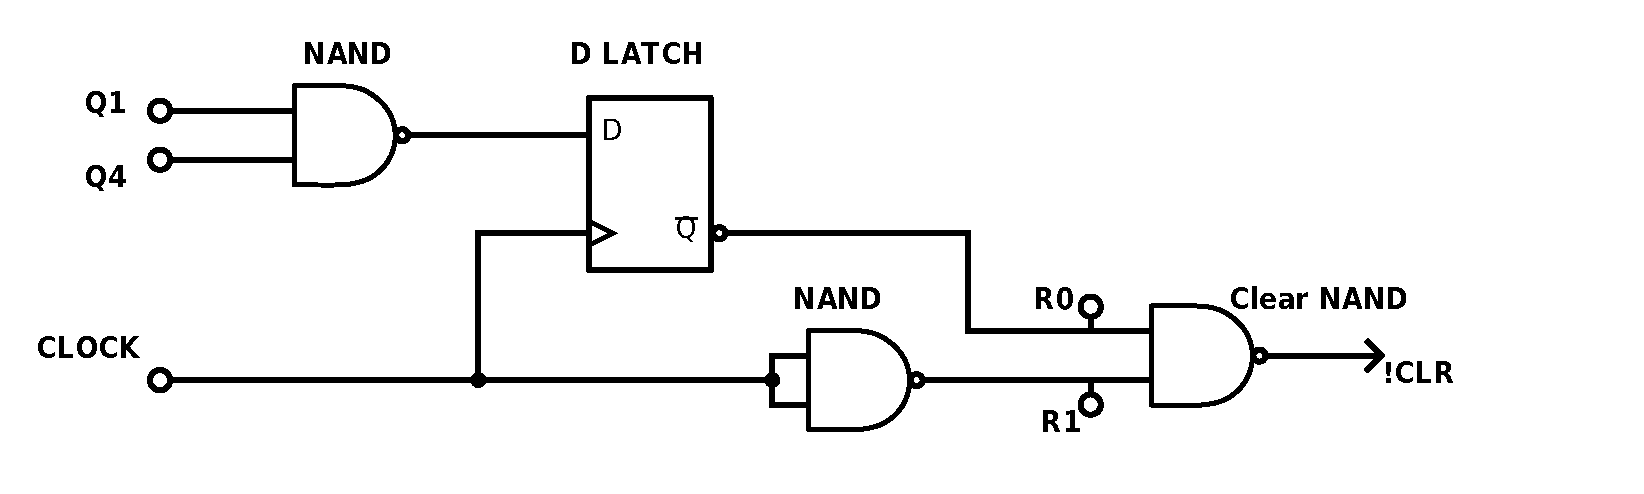
\includegraphics[width=0.9\textwidth]{resetter.pdf}
	\caption{Circuito di reset per il contatore.}
	\label{fig:reset}
\end{figure}

Il D-Latch usato nel circuito di reset è quello realizzato nella sezione precedente dell'esercitazione, sono inoltre state utilizzate altre due porte NAND (la terza è contenuta nell'integrato stesso, con ingressi alle porte 2 e 3). Utilizzare l'output $\overline{Q}$ del D-Latch ci consente di risparmiare una porta NAND, altrimenti necessaria per invertire l'output della prima NAND (l'input del D-Latch).

Il risultato è visibile \fig{div10}, dove qualitativamente si può notare come il segnale in uscita al flip-flop più significativo abbia un periodo pari a 10 periodi di clock (si è anche verificato visivamente attraverso i LED che il comportamento fosse quello atteso); quantitativamente, con un clock a frequenza $f_{clock} = \SI{49.998(1)}{ \kilo \hertz}$ (lo stesso utilizzato nelle misure precedenti) si ottiene in uscita un segnale di frequenza $f_{4} = \SI{4.9999(1)}{ \kilo \hertz}$.

\begin{figure}[h]
	\centering
	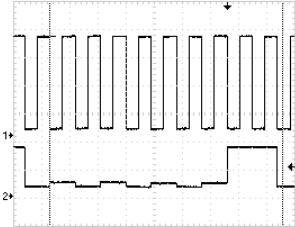
\includegraphics[scale=0.7]{divisore_10x.png}
	\caption{Segnale in uscita al quarto flip-flop del contatore in configurazione divisore 10x.}
	\label{fig:div10}
\end{figure}
